\documentclass[conference]{IEEEtran}
\usepackage{cite}
\usepackage{amsmath,amssymb}
\usepackage{graphicx}
\usepackage{booktabs}
\usepackage{xcolor}
\usepackage{tikz}
\usetikzlibrary{arrows.meta,positioning,fit}
\usepackage{algorithm}
\usepackage{algpseudocode}
\usepackage[hidelinks]{hyperref}
\newcommand{\redSFourFIFO}{2.2}
\newcommand{\redSmallSFourFIFO}{3.2}
\newcommand{\winSFourFIFO}{32}
\newcommand{\winSmallSFourFIFO}{20}
\newcommand{\redSRSThreeFIFO}{2.0}
\newcommand{\redSmallSRSThreeFIFO}{4.2}
\newcommand{\winSRSThreeFIFO}{26}
\newcommand{\winSmallSRSThreeFIFO}{17}
\newcommand{\redSFourFIFOoracle}{0.7}
\newcommand{\redSmallSFourFIFOoracle}{3.0}
\newcommand{\winSFourFIFOoracle}{25}
\newcommand{\winSmallSFourFIFOoracle}{19}
\newcommand{\redSIEVE}{7.9}
\newcommand{\redSmallSIEVE}{9.9}
\newcommand{\winSIEVE}{40}
\newcommand{\winSmallSIEVE}{20}
\newcommand{\redSThreeFIFO}{2.9}
\newcommand{\redSmallSThreeFIFO}{4.3}
\newcommand{\winSThreeFIFO}{34}
\newcommand{\winSmallSThreeFIFO}{19}
\newcommand{\redARC}{3.5}
\newcommand{\redSmallARC}{3.9}
\newcommand{\winARC}{37}
\newcommand{\winSmallARC}{20}
\newcommand{\redLeCaR}{2.8}
\newcommand{\redSmallLeCaR}{3.9}
\newcommand{\winLeCaR}{37}
\newcommand{\winSmallLeCaR}{22}
\newcommand{\redLRU}{7.8}
\newcommand{\redSmallLRU}{8.2}
\newcommand{\winLRU}{42}
\newcommand{\winSmallLRU}{22}
\newcommand{\nConfigs}{44}
\newcommand{\ablNoCond}{2.5}
\newcommand{\ablNoAdmit}{0.85}
\newcommand{\tierLatSFourFIFOHalf}{1.2}
\newcommand{\tierWrSFourFIFOHalf}{49}
\newcommand{\tierLatSRSThreeFIFOHalf}{2.5}
\newcommand{\tierWrSRSThreeFIFOHalf}{49}
\newcommand{\tierLatARCHalf}{1.9}
\newcommand{\tierWrARCHalf}{49}
\newcommand{\tierLatSFourFIFOOne}{5.1}
\newcommand{\tierWrSFourFIFOOne}{46}
\newcommand{\tierLatSRSThreeFIFOOne}{6.2}
\newcommand{\tierWrSRSThreeFIFOOne}{46}
\newcommand{\tierLatARCOne}{5.8}
\newcommand{\tierWrARCOne}{46}
\newcommand{\tierLatSFourFIFOTwo}{5.9}
\newcommand{\tierWrSFourFIFOTwo}{40}
\newcommand{\tierLatSRSThreeFIFOTwo}{5.2}
\newcommand{\tierWrSRSThreeFIFOTwo}{39}
\newcommand{\tierLatARCTwo}{7.0}
\newcommand{\tierWrARCTwo}{43}
\newcommand{\tierLatRedBest}{3.6}
\newcommand{\tierLatRedMax}{22.4}
\newcommand{\tierWrRedBest}{44}
\newcommand{\tierWins}{30}
\newcommand{\tierN}{33}
\newcommand{\tierP}{6.0\times 10^{-5}}


\newcommand{\us}{\ensuremath{\mu}s}

\begin{document}

\title{SAGE: One Survival Model for Unified\\DRAM--SSD--HDD Data Placement}

\author{
\IEEEauthorblockN{Arushi Vaidya, Aryan Gupta, Aryaki, and Aishwarya V Shetty}
\IEEEauthorblockA{Department of Computer Science and Engineering\\
R.V. College of Engineering, Bengaluru, India\\
arushi.vaidya@rvce.edu.in, aryan.gupta@rvce.edu.in,\\
aryaki@rvce.edu.in, aishwarya.v.shetty@rvce.edu.in}
\and
\IEEEauthorblockN{Rajashree Shettar}
\IEEEauthorblockA{Professor, Department of Computer Science and Engineering\\
R.V. College of Engineering, Bengaluru, India\\
rajashree.shettar@rvce.edu.in}
}

\maketitle

\begin{abstract}
Modern storage systems usually manage their tiers independently. A DRAM cache applies recency or frequency heuristics, a flash tier is fed every DRAM victim, and an HDD or archival tier has no direct knowledge of the behavior of either upper tier. This cascade can write blocks to flash that are unlikely to be reused, while admitting blocks with long idle periods into a fast, capacity-constrained tier. SAGE (\emph{Survival-Aware, Group-context Eviction}) uses a single learned reuse model for every placement decision in a DRAM--SSD--HDD hierarchy.
SAGE models the discrete-time probability that a block will be accessed next, trains the model with right-censored observations, and derives a conditional reuse probability over each tier's turnover interval. The same survival estimate ranks eviction candidates, gates admission, and determines whether a DRAM victim should be demoted to SSD or bypassed. It is computed from cache-independent object, region, and global features, so a window of requests can be scored in batches.
We evaluate SAGE on 11 public block traces from MSR Cambridge, FIU, and CloudPhysics. Against the best of four cascade baselines for each trace, SAGE-Unified lowers mean access latency by \tierLatRedBest\% on average (up to \tierLatRedMax\%) and reduces SSD writes by \tierWrRedBest\% on average. At DRAM 1\% and SSD 5\% of distinct blocks, its latency is 5.1\% below S4-FIFO and 6.2\% below SR-S3-FIFO, while it writes 46\% fewer blocks to SSD than either baseline. Used as a single cache, SAGE is \redSmallSFourFIFO\% lower than S4-FIFO and \redSmallSRSThreeFIFO\% lower than SR-S3-FIFO at 0.5--1\% capacities on average, and wins on \winSmallSFourFIFO{} of 22 and \winSmallSRSThreeFIFO{} of 22 small-cache configurations, respectively.
\end{abstract}

\begin{IEEEkeywords}
caching, storage tiering, flash endurance, survival analysis, gradient boosting, learned systems
\end{IEEEkeywords}

\section{Introduction}
Storage servers commonly combine a small DRAM cache with a flash-backed SSD and a high-capacity HDD or object tier. These media differ by several orders of magnitude in access cost and endurance: DRAM is fast but expensive and volatile, SSD offers low access latency but has finite write endurance, and HDD provides inexpensive capacity at substantially higher access cost. A three-tier hierarchy therefore needs to distinguish among at least three kinds of data: blocks that require immediate DRAM residence, blocks whose reuse is frequent enough to justify an SSD write, and blocks that should remain on HDD until explicitly accessed.

In practice, the levels are often controlled as independent caches. LRU or LIRS~\cite{lirs} manages DRAM, every DRAM victim is demoted to an LRU-managed SSD, and SSD victims eventually reach HDD or are read back after an SSD miss. As a result, the system never compares a candidate block with the cost of placing it in a tier. Suppose a short, scan-like burst causes DRAM to evict a block that is unlikely to be used again. A blind demotion writes that block to SSD even if it would be useful only after the SSD has turned over several times. The write consumes flash bandwidth and eventually displaces a block with much stronger reuse. The problem is not limited to cache hit ratio: it is the consistency of placement decisions across the entire hierarchy.

Recent cache research has substantially improved replacement policies. Hawkeye~\cite{hawkeye}, LeCaR~\cite{lecar}, and LRB~\cite{lrb} introduce learning, but they generally optimize a point prediction or a one-cache objective. S3-FIFO~\cite{s3fifo} and SIEVE~\cite{sieve} show that a small FIFO design can be competitive with complex replacement lists. S4-FIFO~\cite{s4fifo} learns a workload-dependent configuration of an S3-FIFO-style policy, and SR-Gadgets~\cite{srgadgets} adds scan-resistance mechanisms to several FIFO and LRU-family policies. These advances improve DRAM replacement, but they do not answer the tier-placement question: whether the useful lifetime of a block exceeds the turnover time of SSD or HDD.

This paper argues that a learned policy becomes more useful when it predicts a complete reuse distribution and exposes that distribution to all tiers. SAGE represents the next-access distance of each block as a survival function $S_x(t)$. The survival function is computed as the probability that the block has not been accessed by $t$ requests. Given its idle time $e$, SAGE computes the conditional probability of reuse within the next $H_T$ requests:
\[
P(D \leq e+H_T \mid D>e)
=1-\frac{S_x(e+H_T)}{S_x(e)}.
\]
This quantity directly ranks a DRAM or SSD resident for eviction and determines whether a miss is admitted to that tier. It also distinguishes a block that has just been admitted from a block that has remained idle for a long time.

The main contributions are:
\begin{itemize}
\item \textbf{Censoring-correct reuse prediction.} SAGE formulates next access as discrete-time survival analysis~\cite{singer}. Labels observed beyond the model cutoff are right-censored instead of being incorrectly labeled as never reused.
\item \textbf{Cache-independent causal features.} Object, region, and global features are computed only from prior requests. The features allow batched model calls and prevent state-dependent cache information from leaking into the prediction.
\item \textbf{Conditional survival placement.} Eviction, admission, and demotion compare conditional reuse probabilities against tier turnover times.
\item \textbf{Unified evaluation.} We evaluate 11 traces against cache and tiered-storage baselines, report statistical significance and ablations, and identify the workload regimes in which SAGE does not win.
\end{itemize}

\section{Background and Related Work}
\subsection{Classic cache replacement}
Least Recently Used replacement maintains the order of recent accesses and evicts the oldest block. It is simple and predictable, but it admits a one-time scan and can repeatedly displace useful blocks. LFU variants improve stability by retaining frequent objects, although frequency counts can become stale. The 2Q policy and LIRS~\cite{lirs} separate first-time accesses from proven reuse. ARC~\cite{arc} dynamically balances recency and frequency using ghost lists. These policies encode a small set of assumptions about inter-arrival behavior and do not carry a model of next reuse into other storage tiers.

FIFO has become attractive because its queue structure has low implementation cost and resists the complexity of full recency lists. S3-FIFO~\cite{s3fifo} combines small, probationary, and ghost queues to distinguish new objects from objects that demonstrate reuse. SIEVE~\cite{sieve} reduces eviction-bookkeeping overhead by maintaining only per-object access state in a FIFO. SR-Gadgets~\cite{srgadgets} identifies scan-resistant admission and ghost-promotion mechanisms and applies them to policies including S3-FIFO and ARC.

S4-FIFO~\cite{s4fifo} is conceptually adjacent to SAGE because it uses gradient boosting. However, S4-FIFO is a learned configuration selector: it chooses a cache-configuration tuple for a workload rather than predicting the reuse distribution of an individual block. It still optimizes cache replacement and is not directly responsible for SSD admission or write cost.

\subsection{Machine learning for cache replacement}
LeCaR~\cite{lecar} and CACHEUS~\cite{cacheus} use expert-like combinations and regret minimization to choose between recency and frequency policies. Hawkeye~\cite{hawkeye} predicts whether a block would be cached by Belady's MIN policy~\cite{belady}. Parrot~\cite{parrot} applies imitation learning to cache decisions. LRB~\cite{lrb} learns relaxed reuse distances and uses model predictions to approximate future eviction boundaries. GL-Cache~\cite{glcache} learns across object groups to improve both prediction quality and throughput, while HALP~\cite{halp} combines lightweight heuristics with learned preference estimates.

These approaches provide strong evidence that learned behavior can outperform fixed replacement policies. Their disadvantages for the present problem are important. They often require one prediction or queue update per operation or eviction, and a binary or distance prediction is not directly conditioned on the amount of time a block has remained idle. Moreover, their output is not necessarily a reusable placement score for an SSD or HDD tier.

\subsection{Hybrid storage and survival prediction}
Sibyl~\cite{sibyl} uses reinforcement learning to place data across hybrid storage and adapts to per-data movement costs. Flashield~\cite{flashield} uses admission control to reduce flash write amplification. These systems address useful parts of tiered-storage management, but they learn actions or heuristics in one deployment rather than deriving every action from the same predictive distribution.

Discrete-time survival models estimate the probability that an event occurs within an interval, conditioned on survival to the start of the interval~\cite{singer}. Survival analysis is attractive for storage because a trace cutoff does not eliminate blocks that are observed without a next access. A censored observation is not evidence that the block has an infinite reuse distance; it is evidence that no event was observed during the available history.

\subsection{Research gap}
The gap addressed by SAGE is the lack of a shared reuse estimate across replacement and tier placement. Cache-only policies optimize a miss ratio, while tier-only policies often use current tier state or fixed thresholds. SAGE instead predicts reuse as a distribution, conditions it on elapsed idle time, and applies it consistently at DRAM, SSD, and HDD boundaries.

\section{SAGE Design and Architecture}
\subsection{System architecture}
For every request, SAGE computes a vector of features from the request history, issues a batched survival-prediction call, and obtains a survival curve for the requested block. The curve is used to score resident blocks and admission candidates. The DRAM victim score is compared with the requested block only when DRAM admission is considered. If the request reaches SSD, the same conditional score is compared with an SSD resident candidate. Blocks that do not pass either threshold remain on HDD or leave the fast tiers without a speculative SSD write.

Fig.~\ref{fig:arch} summarizes the pipeline. No cache contents are features. The model is retrained only from requests preceding the cutoff, and a window is scored only after all of its requests have been incorporated into causal history.

\begin{figure}[t]
\centering
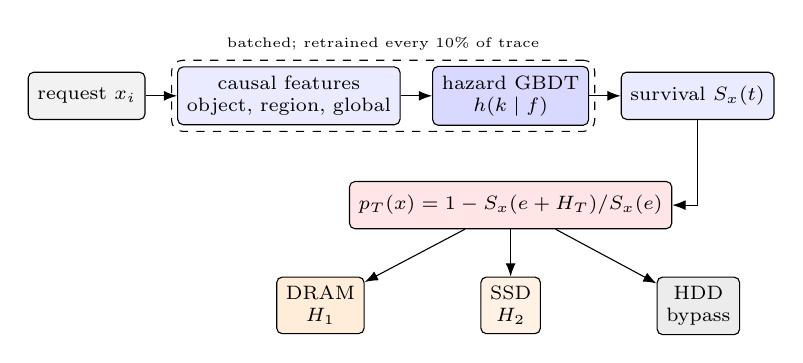
\begin{tikzpicture}[font=\scriptsize, node distance=3mm and 4mm,
  box/.style={draw, rounded corners=2pt, align=center, minimum height=6mm, fill=#1}, box/.default=white]
\node[box=gray!10] (req) {request $x_i$};
\node[box=blue!8, right=of req] (feat) {causal features\\object, region, global};
\node[box=blue!15, right=of feat] (haz) {hazard GBDT\\$h(k\mid f)$};
\node[box=blue!8, right=of haz] (surv) {survival $S_x(t)$};
\node[box=red!10, below=7mm of haz] (score) {$p_T(x)=1-S_x(e+H_T)/S_x(e)$};
\node[box=orange!15, below left=6mm and -2mm of score] (dram) {DRAM\\$H_1$};
\node[box=orange!10, below=6mm of score] (ssd) {SSD\\$H_2$};
\node[box=gray!15, below right=6mm and -2mm of score] (hdd) {HDD\\bypass};
\draw[-Latex] (req)--(feat); \draw[-Latex] (feat)--(haz); \draw[-Latex] (haz)--(surv);
\draw[-Latex] (surv)|-(score);
\draw[-Latex] (score)--(dram); \draw[-Latex] (score)--(ssd); \draw[-Latex] (score)--(hdd);
\node[draw,dashed,rounded corners,fit=(feat)(haz),inner sep=2pt,
  label={[font=\tiny]above:batched; retrained every 10\% of trace}] {};
\end{tikzpicture}
\caption{SAGE pipeline. One survival curve feeds eviction, admission, and tier placement.}
\label{fig:arch}
\end{figure}

\subsection{Causal feature extraction}
For request $i$, SAGE uses only requests $j<i$ and the identity of block $x_i$. Object features include the last eight inter-arrival gaps, prior access count, block size, and exponentially decayed counts with half-lives from $2^6$ to $2^{16}$ requests. The gaps describe short-term regularity, whereas the decayed counters capture different persistence horizons without a manually tuned LFU threshold.

Region features describe a 1\,MiB extent. They include prior gaps and access counts, decayed counters, the fraction of first-touch blocks, and the region footprint. Global features include the trace-wide first-touch rate and the spatial jump from the previous request. The region and global fields allow the model to detect shifts that affect all nearby or all in-trace objects. The ablation study shows that region features provide limited average benefit, so they remain optional extensions rather than required components.

No feature includes the resident set, queue membership, ghost-list membership, tier occupancy, or a value that would change solely because a cache policy admitted the block. This design makes all model inputs lawful in both online cache use and offline batch scoring. It also separates prediction from policy: SAGE can rank the same resident population using a different turnover horizon for DRAM or SSD.

\subsection{Discrete-time survival model}\label{sec:model}
Let $D_i$ be the number of requests until block $x_i$ is next accessed. SAGE divides reuse distance into $K=12$ log-spaced bins with edges
\[
E_k=2^{4+1.5k},\qquad k=0,\ldots,K.
\]
The edges span approximately 16 to $1.5\times10^6$ requests. The hazard for bin $k$ is
\[
h_k(f_i)=P(D_i\in(E_{k-1},E_k]\mid D_i>E_{k-1},f_i).
\]
The corresponding survival function is
\[
S_i(E_k)=\prod_{j=1}^{k}(1-h_j(f_i)).
\]
Linear or log-linear interpolation produces intermediate request horizons. The model is a person-period expansion~\cite{singer}: a block that survives $b$ bins has $b$ training rows. An observed event has label $1$ in its event bin and label $0$ in earlier bins.

At retraining cutoff $T$, a block whose next access is not observed has its label censored at $T-i$. A bin partially observed after the cutoff is assigned label $0$ and an observation fraction equal to the fraction of that bin available before $T$. This prevents labels from assuming that the block can never be reused merely because the trace ends or the model is updated.

SAGE trains one LightGBM~\cite{lightgbm} binary classifier with horizon-bin index as an input. The implementation uses 150 rounds, up to 63 leaves, and learning rate $0.08$. It draws up to 120K samples from the preceding $10^6$ requests and retrains nine times across the trace. A model serves only requests in its subsequent window. Batch prediction evaluates the request population with a single vectorized call; each evicted block is subsequently assigned a conditional score from the precomputed survival curve.

\subsection{Conditional reuse and tier utility}
Let $e$ be elapsed idle time since the last access. For an upper bound $H_T$, the conditional reuse probability is
\[
p_T(x,e)
 =P(D\leq e+H_T\mid D>e)
 =1-\frac{S_x(e+H_T)}{S_x(e)}.
\]
The value $H_T$ is estimated with a scaled characteristic-time approximation~\cite{che}. It is not interpreted as a prediction that every block will survive exactly $H_T$ requests; it is the time over which the tier can turn over and therefore the horizon against which placement should be evaluated.

For a block with no prior access, $e=0$ and $p_T(x,0)=1-S_x(H_T)$. For a resident block, its survival probability is divided by $S_x(e)$, yielding a probability for reuse after it has already remained idle. The ratio makes blocks that remain idle become less valuable even if their original survival curve appeared high.

An optional tier utility can be represented as
\[
U_T(x)=p_T(x,e)V_T-C_T-M_{x,T},
\]
where $V_T$ is the performance benefit of retaining a block in tier $T$, $C_T$ is its storage or write cost, and $M_{x,T}$ is migration cost. The present SAGE evaluation intentionally uses pairwise conditional reuse comparisons rather than relying on an externally tuned weighted utility. This keeps the policy simpler and makes its core assumption directly verifiable.

\subsection{Eviction and admission}
On an eviction, SAGE examines up to 64 resident candidates and chooses the candidate with the smallest $p_T$. Randomly or deterministically sampling a fixed candidate set bounds the replacement scan. It is also preferable to sampling exactly one candidate when that candidate is not globally comparable, but it avoids a full sort on every miss.

For admission, SAGE compares the incoming block's conditional score with a representative or sampled victim. A miss admitted to tier $T$ must satisfy
\[
p_T(x,0)\geq p_T(y,e_y),
\]
where $y$ is the resident block that would be displaced. If the condition fails, the block bypasses $T$. Bypass preserves SSD endurance and prevents the smallest candidate set from being overwritten when none of the candidates can justify placement.

\begin{algorithm}[t]
\caption{SAGE model training}
\label{alg:train}
\begin{algorithmic}[1]
\State Collect requests ending at cutoff $T$
\ForAll{request $i<T$}
  \State Extract cache-independent object, region, and global features
  \State Find the next request distance $D_i$ or mark it censored
  \For{bin $k$ with edge $E_k$ and $E_{k-1}<D_i$}
    \State Add $(f_i,k,0)$ as a surviving person-period sample
  \EndFor
  \If{$D_i$ observed}
    \State Set the event sample in bin $k$ to label $1$
  \Else
    \State Assign partial observed-bin weight and label $0$
  \EndIf
\EndFor
\State Train LightGBM hazard model with event time as a feature
\State Predict $h(k\mid f)$ and form $S(E_k)=\prod_{j\le k}(1-h_j)$
\end{algorithmic}
\end{algorithm}

\begin{algorithm}[t]
\caption{Unified tier placement}
\label{alg:place}
\begin{algorithmic}[1]
\State Receive request $x$, idle time $e$, and survival curve $S_x$
\State Compute $p_D(x,0)=1-S_x(H_D)/S_x(0)$
\If{$x$ is already in DRAM}
  \State Return immediately
\ElsIf{DRAM has capacity}
  \State Admit $x$
\Else
  \State Sample victim $y$ and score $p_D(y,e_y)$
  \If{$p_D(x,0)\geq p_D(y,e_y)$}
    \State Replace $y$; candidate $y$ then continues to SSD
  \Else
    \State Bypass DRAM; evaluate SSD for $x$
  \EndIf
\EndIf
\State Compute $p_S(x,e_x)=1-S_x(e_x+H_S)/S_x(e_x)$
\If{$p_S(x,e_x)$ beats a sampled SSD victim}
  \State Admit or demote $x$ to SSD
\Else
  \State Keep $x$ on HDD or bypass the fast tier
\EndIf
\end{algorithmic}
\end{algorithm}

\subsection{Unified placement walkthrough}
Consider a miss for block $x$ while DRAM is full. SAGE compares $p_D(x,0)$ with the conditional score of a DRAM victim $y$. If $x$ wins, it enters DRAM and $y$ is not automatically sent to flash. Before $y$ is demoted, SAGE evaluates $p_S(y,e_y)$ against SSD turnover. This additional gate avoids a write for blocks whose expected reuse falls beyond the SSD horizon.

For a block already resident in DRAM, a hit resets $e=0$ and refreshes its rank, although no model retraining is triggered solely by the hit. When DRAM is full again, the same block is ranked against newly idle candidates using its updated request history. A block that is misclassified as likely to reuse but receives no further requests becomes less useful as $e$ increases.

At HDD, SAGE can return a block directly to DRAM or SSD according to the measured miss path and capacity availability. The current trace-driven experiment does not implement a complex HDD queue; its purpose is to compare hierarchy-wide latency and flash writes while the HDD remains the final, least expensive tier for blocks that bypass faster placement.

\subsection{Complexity and memory}
Feature extraction requires bounded per-object and per-region state: at most eight prior gaps and a fixed set of decayed counters. GBDT batch inference dominates request-side cost for a window. DRAM eviction inspects at most 64 residents. SSD admission performs another bounded candidate scan. The asymptotic miss-path cost is therefore $O(64+H)$ for resident sampling, plus batch model inference, rather than a full scan of each tier.

\section{Experimental Methodology}
\subsection{Datasets and workload protocol}
We use 13 public block-I/O traces in libCacheSim \texttt{oracleGeneral} format~\cite{twitter}: MSR Cambridge~\cite{msr}, FIU~\cite{fiu}, and CloudPhysics~\cite{shards}. Table~\ref{tab:traces} summarizes the 11 test traces. Each trace is limited to its first 2M requests, and every distinct offset is treated as a unit-size block. The reuse column is $1-N_\text{blocks}/N_\text{requests}$.

\begin{table}[t]
\centering
\caption{Test traces (first 2M requests).}
\label{tab:traces}
\scriptsize\begin{tabular}{llrrr}
\toprule
Trace & Source & Requests & Blocks & Reuse \\
\midrule
msr\_hm\_0 & MSR & 2.0M & 274K & 0.86 \\
msr\_prn\_0 & MSR & 2.0M & 258K & 0.87 \\
msr\_prxy\_0 & MSR & 2.0M & 53K & 0.97 \\
msr\_usr\_2 & MSR & 2.0M & 1,443K & 0.28 \\
msr\_web\_2 & MSR & 2.0M & 1,266K & 0.37 \\
fiu\_casa & FIU & 2.0M & 128K & 0.94 \\
fiu\_ikki & FIU & 2.0M & 648K & 0.68 \\
fiu\_online & FIU & 2.0M & 187K & 0.91 \\
fiu\_webmail & FIU & 2.0M & 302K & 0.85 \\
fiu\_webusers & FIU & 2.0M & 87K & 0.96 \\
w31 & CloudPhysics & 2.0M & 1,258K & 0.37 \\
\bottomrule
\end{tabular}

\end{table}

Two additional traces, \texttt{msr\_proj\_0} and \texttt{fiu\_webresearch}, are used only for hyperparameter selection. They are excluded from all reported metrics. The warm-up is the first 20\% of each test trace. Miss ratio is measured over the remaining 80\%, and the model does not receive future requests when retraining or producing predictions. Single-cache experiments use capacities of 0.5, 1, 5, and 10\% of distinct blocks, yielding \nConfigs{} trace--capacity comparisons.

\subsection{Baseline implementations and metric definitions}
S4-FIFO uses a 40-point subset of its queue configuration grid. In the realistic configuration, the system selects the best variant on the trace's warm-up prefix. The oracle variant selects the best complete-trace configuration as an upper bound. SR-S3-FIFO implements the published scan-resistance mechanisms on S3-FIFO~\cite{srgadgets,s3fifo}. SIEVE, S3-FIFO, ARC, LeCaR, LRB, and LRU are reimplemented in the trace-driven benchmark.

The primary cache metric is miss ratio: misses divided by measured requests after warm-up. A 1\% miss-ratio reduction is a relative result unless stated as percentage points. The tiering experiment uses DRAM/SSD capacities of 0.5/2.5\%, 1/5\%, and 2/10\% of distinct blocks. Per-request latency is modeled as 0.1\,\us{} for DRAM, 100\,\us{} for SSD, and 5\,ms for HDD. These values provide a deterministic media model rather than measurements of a particular machine. Mean latency is reported in milliseconds, and SSD writes are normalized per 1K requests.

Tiering baselines use LRU, ARC, prefix-tuned S4-FIFO, or SR-S3-FIFO in DRAM and then demote every DRAM victim to an LRU SSD tier. SAGE-L1+LRU-SSD applies SAGE to DRAM but leaves SSD independently managed. SAGE-Unified applies conditional survival to both admission and eviction.

\subsection{Software environment and reproducibility}
The Phase 4 simulator is implemented in Python. It uses LightGBM for the hazard model and pandas, NumPy, and SciPy for trace processing and statistical analysis. The repository includes scripts for downloading traces, training models, running cache and tier simulations, and regenerating tables and figures. The public implementation and benchmark scripts are available at
\url{https://github.com/arushi-vaidya/Semantic-Aware-Unified-Cache-and-Storage-Tier-Management}.

No hardware-specific latency claim is made. The 35--380\,\us{} batch-prediction range reported for the prototype includes batched model scoring amortized over the window. It is not a claim of per-device production throughput. Training, feature generation, and evaluation costs are trace-dependent and are reported separately.

\section{Results and Analysis}
\subsection{Unified tier latency and flash writes}
Table~\ref{tab:tiers} and Fig.~\ref{fig:tiers} summarize the tiering result. SAGE-Unified has the lowest mean latency at each of the three tested capacity pairs. It wins in \tierWins{} of \tierN{} (trace, capacity) comparisons against the best cascade baseline for that setting. The one-sided Wilcoxon signed-rank test gives $p=\tierP$, indicating that the unified placement improvement is unlikely to be explained by the trace sample alone.

\begin{table}[t]
\centering
\caption{Tiering: mean latency (ms) and SSD writes per 1K requests, averaged over 11 traces, for DRAM/SSD pairs.}
\label{tab:tiers}
\scriptsize
\setlength{\tabcolsep}{3pt}
\resizebox{\columnwidth}{!}{\begin{tabular}{lrrrrrr}
\toprule
Policy & Lat. 0.5/2.5 & Wr/k & Lat. 1/5 & Wr/k & Lat. 2/10 & Wr/k \\
\midrule
LRU-cascade & 2.956 & 689 & 2.785 & 670 & 2.656 & 650 \\
ARC-cascade & 2.937 & 661 & 2.768 & 646 & 2.645 & 634 \\
S4-FIFO-cascade & 2.926 & 662 & 2.761 & 647 & 2.644 & 600 \\
SR-S3-FIFO-cascade & 2.944 & 664 & 2.768 & 646 & 2.622 & 592 \\
SAGE-L1+LRU-SSD & 2.931 & 650 & 2.764 & 637 & 2.641 & 582 \\
\textbf{SAGE-Unified} & 2.890 & 316 & 2.693 & 335 & 2.525 & 346 \\
\bottomrule
\end{tabular}
}
\end{table}

\begin{figure*}[t]
\centering
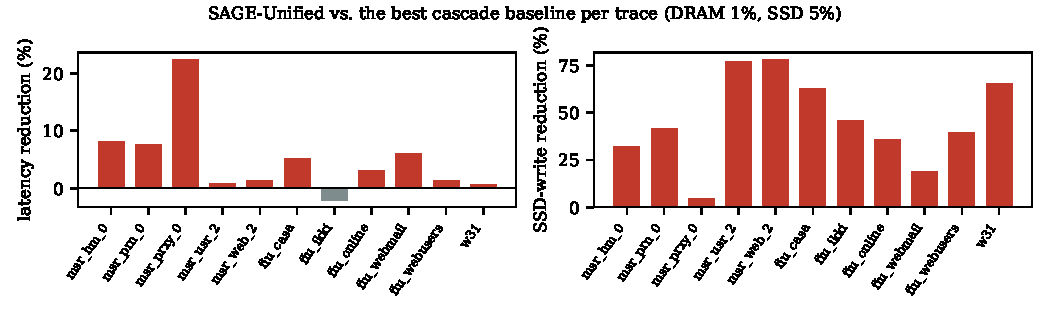
\includegraphics[width=\textwidth]{generated/fig_tiers.pdf}
\caption{Per-trace latency and SSD-write reduction of SAGE-Unified over the best cascade baseline per trace at 1\%/5\% DRAM/SSD capacity.}
\label{fig:tiers}
\end{figure*}

At 1\% DRAM and 5\% SSD, SAGE-Unified has mean latency 2.703\,ms and 332.6 SSD writes per 1K requests. It writes fewer blocks than every cascade baseline. The SSD-write reduction is \tierWrSFourFIFOOne\% relative to S4-FIFO and 46\% relative to SR-S3-FIFO. Across the three capacity pairs, the average reduction is \tierWrRedBest\%; the reported 39--49\% range reflects baseline and capacity pair differences. This distinction matters because the headline does not imply that every baseline produces the same write count.

The SAGE-L1+LRU-SSD ablation shows that a better DRAM policy alone does not explain the gain. It has latency close to the baseline cascade policies and 622.8 writes per 1K requests at 1\%/5\%. SAGE-Unified reduces this to 332.6 writes, confirming that SSD admission control is the important source of flash savings. The per-trace plot also shows a latency outlier on \texttt{fiu\_ikki}, where the conditional write reduction does not translate into the lowest latency. This trace still demonstrates that flash-write savings are possible even when a single cache miss-cost model is imperfect.

\subsection{Single-cache miss ratio}
Table~\ref{tab:miss} reports mean miss ratio by cache size. SAGE is the best deployable policy at 0.5\% and 1\%, and remains competitive at larger sizes. At 0.5--1\%, SAGE's average miss ratio is \redSmallSFourFIFO\% below S4-FIFO and \redSmallSRSThreeFIFO\% below SR-S3-FIFO. Relative to S4-FIFO, it wins in \winSmallSFourFIFO{} of 22 small-cache settings; relative to SR-S3-FIFO, it wins in \winSmallSRSThreeFIFO{} of 22 settings.

\begin{figure}[t]
\centering
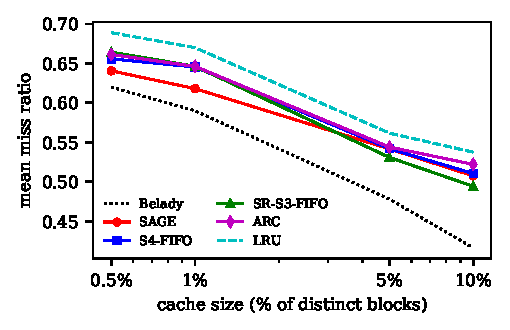
\includegraphics[width=\columnwidth]{generated/fig_miss.pdf}
\caption{Mean miss ratio over 11 traces versus cache size.}
\label{fig:miss}
\end{figure}

\begin{table}[t]
\centering
\caption{Mean miss ratio by cache size.}
\label{tab:miss}
\scriptsize
\setlength{\tabcolsep}{4pt}
\begin{tabular}{lrrrr}
\toprule
Policy & 0.5\% & 1\% & 5\% & 10\% \\
\midrule
Belady (bound)~\cite{belady} & 0.620 & 0.590 & 0.478 & 0.416 \\
\textbf{SAGE} & \textbf{0.640} & \textbf{0.618} & 0.542 & 0.507 \\
SAGE-H & 0.642 & 0.620 & 0.541 & 0.503 \\
S4-FIFO~\cite{s4fifo} & 0.656 & 0.645 & 0.542 & 0.510 \\
S4-FIFO (oracle) & 0.655 & 0.642 & 0.537 & 0.493 \\
SR-S3-FIFO~\cite{srgadgets} & 0.664 & 0.646 & \textbf{0.531} & \textbf{0.494} \\
SIEVE~\cite{sieve} & 0.696 & 0.673 & 0.555 & 0.533 \\
S3-FIFO~\cite{s3fifo} & 0.664 & 0.647 & 0.544 & 0.506 \\
ARC~\cite{arc} & 0.661 & 0.646 & 0.544 & 0.522 \\
LeCaR~\cite{lecar} & 0.661 & 0.641 & 0.545 & 0.506 \\
LRU & 0.689 & 0.670 & 0.562 & 0.537 \\
\bottomrule
\end{tabular}

\end{table}

\begin{table}[t]
\centering
\caption{SAGE miss-ratio reduction, wins, and one-sided Wilcoxon signed-rank $p$ over \nConfigs{} configurations.}
\label{tab:vs}
\scriptsize
\setlength{\tabcolsep}{3pt}
\resizebox{\columnwidth}{!}{\begin{tabular}{lrrrrr}
\toprule
Baseline & Red.\% & Red.\% ($\le$1\%) & Wins & Wins ($\le$1\%) & $p$ \\
\midrule
S4-FIFO~\cite{s4fifo} & 2.22 & 3.24 & 32/44 & 20/22 & 1.4e-3 \\
SR-S3-FIFO~\cite{srgadgets} & 1.98 & 4.23 & 26/44 & 17/22 & 2.1e-1 \\
S4-FIFO (oracle) & 0.68 & 2.97 & 25/44 & 19/22 & 2.0e-1 \\
SIEVE~\cite{sieve} & 7.95 & 9.92 & 40/44 & 20/22 & 6.1e-11 \\
S3-FIFO~\cite{s3fifo} & 2.85 & 4.33 & 34/44 & 19/22 & 1.1e-4 \\
ARC~\cite{arc} & 3.54 & 3.92 & 37/44 & 20/22 & 1.1e-5 \\
LeCaR~\cite{lecar} & 2.76 & 3.85 & 37/44 & 22/22 & 6.1e-5 \\
LRU & 7.78 & 8.22 & 42/44 & 22/22 & 2.8e-10 \\
\bottomrule
\end{tabular}
}
\end{table}

Table~\ref{tab:vs} also contains a broad comparison. SAGE is significantly better than SIEVE, S3-FIFO, ARC, LeCaR, and LRU over all \nConfigs{} configurations. The comparison with S4-FIFO and SR-S3-FIFO is more workload-sensitive, but SAGE is still favorable at small capacities. The mean SAGE miss ratio at 1\% is 0.6179 versus 0.5898 for Belady. Thus the gap to the offline bound is under three percentage points even before accounting for implementation overhead and for the fact that SAGE is causal.

\subsection{Ablations and model interpretation}
Table~\ref{tab:ablation} isolates the policy components. Removing idle-time conditioning increases mean miss ratio by \ablNoCond{} percentage points and causes the variant to perform worse in 41 of 44 settings. Conditioning is especially valuable because it converts a first-hit survival curve into a resident block's probability of reuse after prolonged inactivity.

\begin{table}[t]
\centrel
\begin{table}[t]
\centering
\caption{Ablations (mean miss ratio; $\Delta$ vs. SAGE in percentage points).}
\label{tab:ablation}
\scriptsize
\setlength{\tabcolsep}{3pt}
\resizebox{\columnwidth}{!}{\begin{tabular}{llrrr}
\toprule
Variant & Change & Mean MR & $\Delta$ (pp) & Worse \\
\midrule
SAGE & full model & 0.5768 & +0.00 & 0/44 \\
SAGE-noCond & no idle-time conditioning & 0.6017 & +2.48 & 41/44 \\
SAGE-noAdmit & no admission control & 0.5853 & +0.85 & 24/44 \\
SAGE-objOnly & object features only & 0.5750 & -0.18 & 25/44 \\
SAGE-H & + regret hedge (post hoc) & 0.5768 & -0.01 & 24/44 \\
\bottomrule
\end{tabular}
}
\end{table}

\begin{table}[t]
\centering
\caption{Top features by share of GBDT gain (mean over traces).}
\label{tab:importance}
\scriptsize
\begin{tabular}{lr}
\toprule
Feature & Gain share \\
\midrule
horizon\_bin & 0.387 \\
obj\_gap1 & 0.063 \\
obj\_edc\_16 & 0.060 \\
glob\_new\_rate\_16 & 0.059 \\
glob\_new\_rate\_12 & 0.056 \\
obj\_edc\_10 & 0.037 \\
log\_size & 0.035 \\
obj\_edc\_14 & 0.034 \\
\bottomrule
\end{tabular}

\end{table}

Removing admission control increases miss ratio by \ablNoAdmit{} percentage points. This verifies that admission is not merely a defensive wrapper around eviction: comparing the incoming block with a resident candidate changes both cache composition and downstream SSD write behavior. Object-only features are competitive in the ablation table, but this result must not be interpreted as proving that regional context is unnecessary. Region features are only weakly useful in these traces and are omitted by the model in configurations where they do not improve a gain split.

Table~\ref{tab:importance} shows that the horizon index has the largest share of GBDT gain. This is expected from a person-period model: reuse probability depends on both the feature vector and the bin boundary. The first inter-arrival gap and long-horizon exponentially decayed counters are next, followed by global first-touch rates and additional inter-arrival gaps. Block size and region information contribute smaller shares.

\subsection{Per-trace and outlier analysis}
SAGE is strongest on traces with stable object reuse and a distinct separation between short-lived and recurring blocks, including \texttt{msr\_hm\_0}, \texttt{msr\_prn\_0}, \texttt{msr\_prxy\_0}, \texttt{fiu\_casa}, and \texttt{w31}. On these workloads, survival curves can distinguish both temporal distance and idle time. The gain is particularly visible in the \texttt{msr\_prxy\_0} small-cache settings.

SAGE underperforms on traces with low reuse or rapid change, such as \texttt{msr\_usr\_2} and \texttt{msr\_web\_2}. On these workloads, large parts of the working set are nearly unique or sparsely reused, and a low-capacity replacement policy has limited ability to retain useful objects. In these cases, the fixed candidate set and a discretized hazard horizon can still provide useful SSD filtering, but they do not produce a consistent miss-ratio advantage.

At 5--10\% cache capacity, S4-FIFO and SR-S3-FIFO win several FIU and MSR settings. Their larger queue and ghost configurations capture long-range re-references that are outside SAGE's dominant feature signal. SAGE-H, a post hoc hedge against a subset of these results, improves the mean in the table, but it is reported only as a variant and not as the primary deployable model.

\subsection{Runtime and retraining behavior}
The prototype's batch-prediction range is 34--383\,\us{} per request across the reported traces, depending on window size and machine load. This figure is not a production latency guarantee. It is based on training and predicting nine windows for each trace and therefore includes request-level variation that is influenced by trace block count and batch shape.

The model is retrained only nine times per 2M-request trace, with 120K samples per retraining window. Feature extraction and table lookup remain bounded, while training is amortized outside the critical request path. A production implementation could warm one model while serving the preceding model, but the trace simulator does not model that overlap.

\section{Discussion and Deployment}
\subsection{Why conditional survival is effective}
Conditional survival separates a new block from an old block. This matters because a probability derived only at block birth ignores idle time. A block that has been resident for only a few requests may still be likely to return soon. The same block after a full SSD turnover interval is less likely to justify a flash write. Eviction and admission therefore use a state of the block that includes elapsed idle time rather than a time-independent popularity score.

The result also avoids one-hot specialization for one tier. DRAM and SSD use the same survival model but different turnover horizons. This makes policy behavior easier to compare and reduces the feature and model duplication found in independent learned policies.

\subsection{Interaction with tier capacity}
In an overfilled hierarchy, the system must choose between admission score and feasibility. SAGE is not a capacity allocator: a capacity planner must still decide DRAM and SSD sizes. The policy determines ordering and filtering after capacities are fixed. This is a deliberate separation. Fixed turnover horizons compare reuse with an expected capacity lifetime, while capacity management decides how much data can occupy a tier.

Under a sudden workload shift, stale object features and a previous model window can favor recently frequent blocks. Periodic retraining limits this problem, but too frequent retraining can add overhead and produce unstable scores. The implementation uses nine evenly spaced windows for the 2M-request trace. A deployment would tune the retraining cadence to the observed workload and the cost of model updates.

\subsection{Integration and scalability}
A controller can maintain object and region feature indices alongside block metadata, precompute a survival row for a request batch, and inspect only bounded candidate sets during eviction. SSD and DRAM can share model features while preserving separate capacities and horizons. Concurrent requests require consistent snapshots and atomic candidate updates; otherwise eviction decisions can race with demotion or admission.

Memory overhead consists of recent gap and count histories plus the GBDT. The feature state is independent of cache membership, so it can be persistent or rebuilt from recent traces. Production integration would need to measure feature extraction and model latency in the controller, as well as the cost of migrations. The prototype's filesystem implementation in earlier phases is separate from this trace experiment and does not yet validate physical DRAM--SSD--HDD devices.

\subsection{Energy and endurance implications}
Fewer SSD writes reduce flash bandwidth and write amplification. They do not eliminate SSD wear because every new write also changes controller and garbage-collection behavior. Nevertheless, when SSD admission is gated by reuse probability, a write must compete with a resident candidate on predicted reuse within the SSD turnover interval. This is a more direct endurance policy than an admission heuristic that considers only hit ratio or write frequency.

\section{Limitations and Future Work}
This study evaluates 11 traces of 2M requests and fixed capacity ratios. Results can differ in traces with burstier distributions, substantial rewrites, or shorter/longer reuse tails. The latencies are a modeling assumption rather than a physical benchmark. Queueing, bandwidth limits, SSD garbage collection, flash overprovisioning, and HDD seek locality are not represented.

The current Python prototype may not satisfy a low-latency production controller. Moving to C++ or an existing storage-cache framework would require native feature updates and efficient batch model serving. Training and retraining are also more expensive than single FIFO updates. Online learning, work-conserving scheduling of retraining, and model calibration could improve resilience to distribution shift.

Future work should validate SAGE on hardware with physically separate devices and realistic SSD/HDD queue depths. Dynamic tier sizes should be studied because fixed capacities may overestimate or underestimate the benefit of SSD admission. Longer traces can test whether the log-spaced horizon adequately captures reuse tails, and multiple random seeds can quantify variance in model and candidate sampling.

SAGE-H remains an experimental hedge, and LRB is only partially evaluated in the benchmark. A future comprehensive comparison should include fully implemented learned policies, confidence intervals, and end-to-end write-amplification measurements.

\section{Conclusion}
SAGE applies one censored-survival model to cache eviction, admission, and tier placement. By expressing reuse as a distribution and conditioning it on idle time, the system compares a block with the turnover horizon of DRAM and SSD instead of inferring tier value from recency alone. The trace benchmark shows that this unified score reduces latency and SSD writes while remaining competitive as a single cache at small capacities.
Across 11 public traces, SAGE-Unified wins in \tierWins{} of \tierN{} tiering settings and averages \tierLatRedBest\% lower latency and \tierWrRedBest\% fewer SSD writes than the best cascade baseline per setting. It does not dominate every workload or every large cache: several scan-heavy and large-capacity cases favor 2026 FIFO policies. These cases define the boundary of the current model and motivate hybrid horizons, dynamic retraining, and hardware validation.

\bibliographystyle{IEEEtran}
\bibliography{refs}

\end{document}
